\documentclass[times]{article}

\usepackage[margin=1.0in]{geometry}
\usepackage{graphicx}
\usepackage{adjustbox}
\usepackage{float}
\usepackage{placeins}
\usepackage[none]{hyphenat}
\usepackage{amsmath}
\usepackage[us]{datetime}
\usepackage[explicit]{titlesec}
\usepackage{standalone}
\maxdeadcycles=100000
\begin{document}
	\title{”COMP SCI 5401 FS2017 Assignment 2c}
	\author{Dalton Cole \\ drcgy5@mst.edu}
	\date{\formatdate{3}{12}{2017}}
	\maketitle

	\section{Methodology}

	\section{Experimental Setup}

	\section{Results}

	\section{Discussion}

	\section{Conclusion}

	\section{Bonus 1}

	\section{bonus 2}

	Methodology section 10
Experimental setup section 5
Results section 10
Discussion section 10
Conclusion section 

	\section{Genetic Programming Search}
	For this experiment, implementing a genetic programming search of the Prisoner's Dilemma was required. Evaluations vs Fitness Plot can be seen in Figure \ref{fig:plot}.

	As seen in Figure \ref{fig:stat}, genetic programming search out performs random search.

	\begin{figure}
		\caption{Eval vs Fitness Plot}
		\label{fig:plot}
		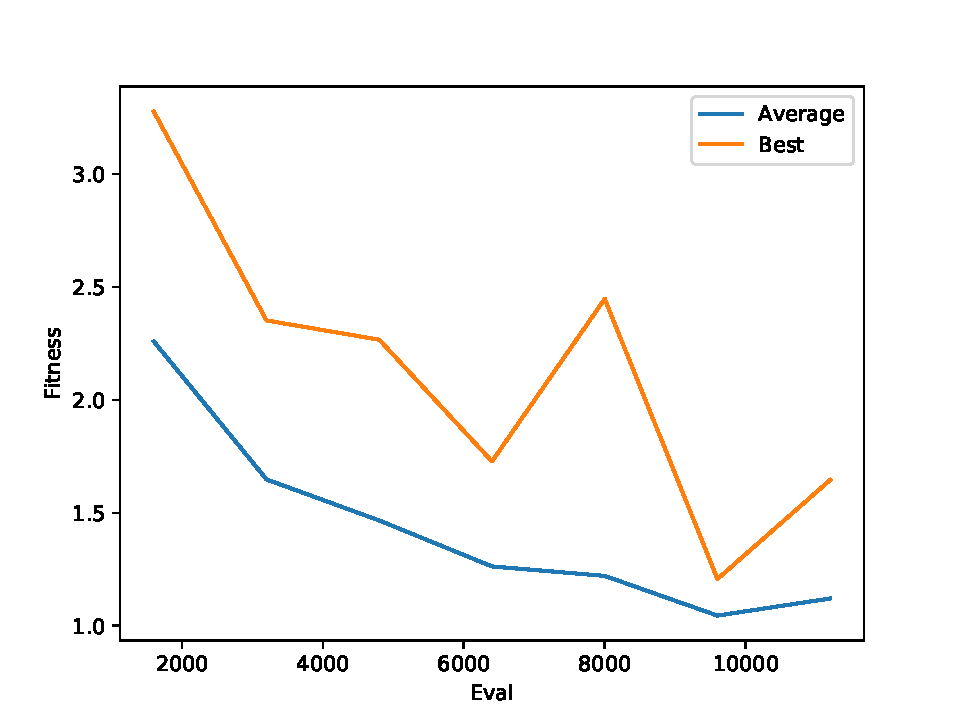
\includegraphics[width=\textwidth]{../graph/graphs/0.pdf}
	\end{figure}

	\begin{figure}
		\caption{Statistical Analysis}
		\label{fig:stat}
		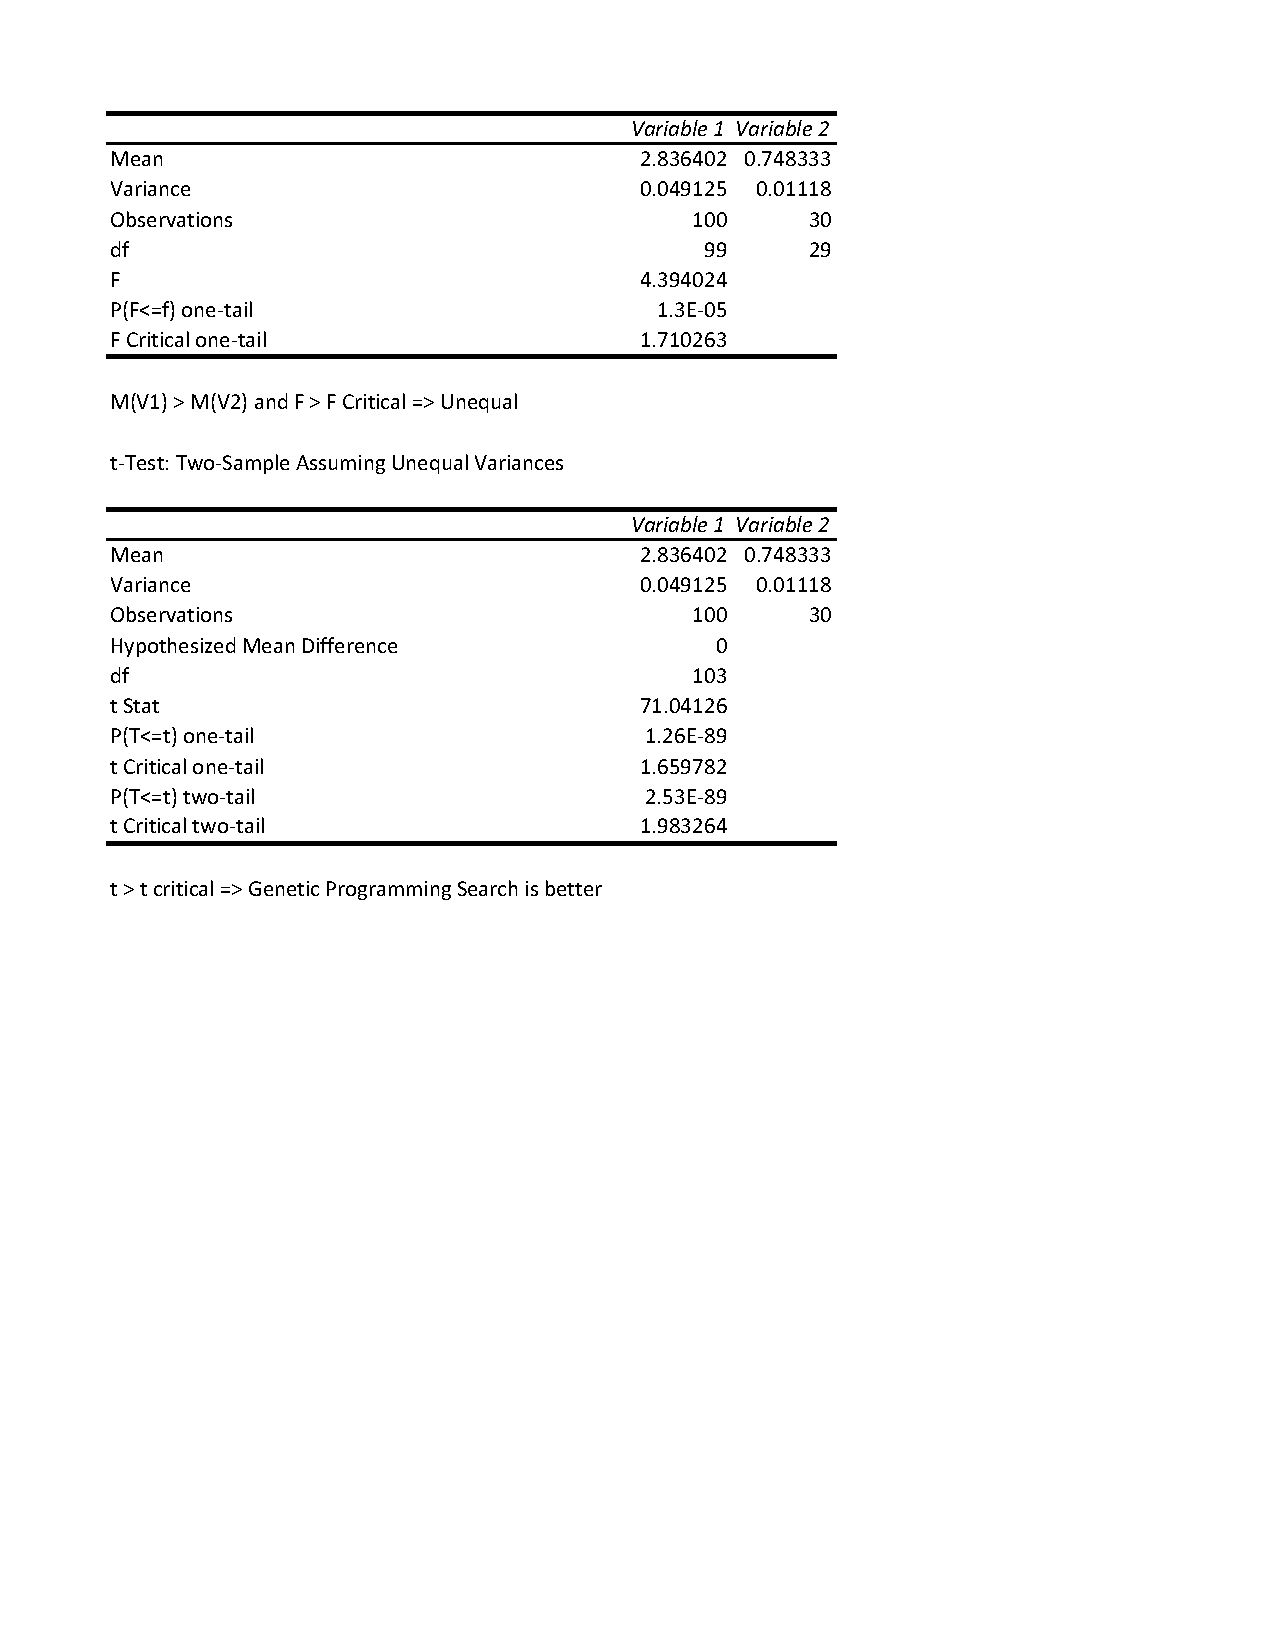
\includegraphics[width=\textwidth]{./pictures/test.pdf}
	\end{figure}


		
\end{document}
